\section{Methods and Results} 
\label{sec:taxonomy}
%% \stodor{Combines \textbf{Data Description} + \textbf{Analyses} + \textbf{Methods}; \url{https://academic.oup.com/gigascience//pages/research}}
Because metadata captured in ROs should be able to fulfill provenance requirements of real workflows, identification of these requirements is crucial to understand which metadata should be collected during execution, either by the workflow system or via manual annotations. However, due to the large variety of scientific communities and workflows, it is unlikely that a universal standard for which to capture exists which is still sufficiently detailed to capture domain-specific elements. 
% Defining a standard for provenance which is detailed enough to fulfill domain-specific requirements, yet general enough to be relevant across a broad range of scientific disciplines is challenging. 

Instead, we restricted ourselves to the detailed analysis of a single exemplary bioinformatics workflow, and formulated specific \emph{provenance questions} grounded in a set of realistic use case scenarios.
% Here, we approach this problem by examining one example real-life workflow in detail and identifying elements of the analysis that are relevant in one of the potential \emph{use case scenarios} for ROs associated with it. The resulting \emph{provenance taxonomy}
This imagination exercise gave us much insight into a set of important provenance metadata, and, summarizing it into a \emph{provenance taxonomy}, we studied the representation of each component of the taxonomy in the current CWLProv community standard. 
% \stodor{Which "its" was studied?}
Our analysis revealed that some elements of the taxonomy were insufficiently described, and that others were dependent on manual annotations of the input data and the workflow descriptions itself (for which the CWL standards were insufficiently clear); therefore our final step was to design extensions to CWLProv and guidance on manual annotations to address the gaps we had identified. 

% In summary, we take an example workflow in the field of bioinformatics and define a number of associated \emph{use case scenarios} for the results generated by one of its enactments. We synthesize a list of \emph{provenance questions} associated with each of the use cases and identify components of the analysis that should be described in the provenance record in order to answer the provenance questions. Subsequently, we classify these elements into a 6-component \emph{provenance taxonomy}. 

The rest of this section is organized as follows. Firstly, we describe the design and implementation of our exemplary workflow in CWL. Secondly, we define five realistic use case scenarios for ROs associated with the workflow. Subsequently, we synthesize a provenance taxonomy, based on a list of provenance questions grounded in each of the RO use case scenarios. Next, we describe the approach and results of our qualitative analysis of the current version of CWLProv (v0.6.0). Finally, we propose the design of two extensions to CWLProv: a scheme for annotation of workflow input data, and an extension of the provenance graph to enrich the RDF representation of the workflow execution. 

\subsection{Design and implementation of an exemplary bioinformatics workflow}
\label{sec:workflow}
\begin{figure*}[hb!]
    \label{fig:epitope_graph}
    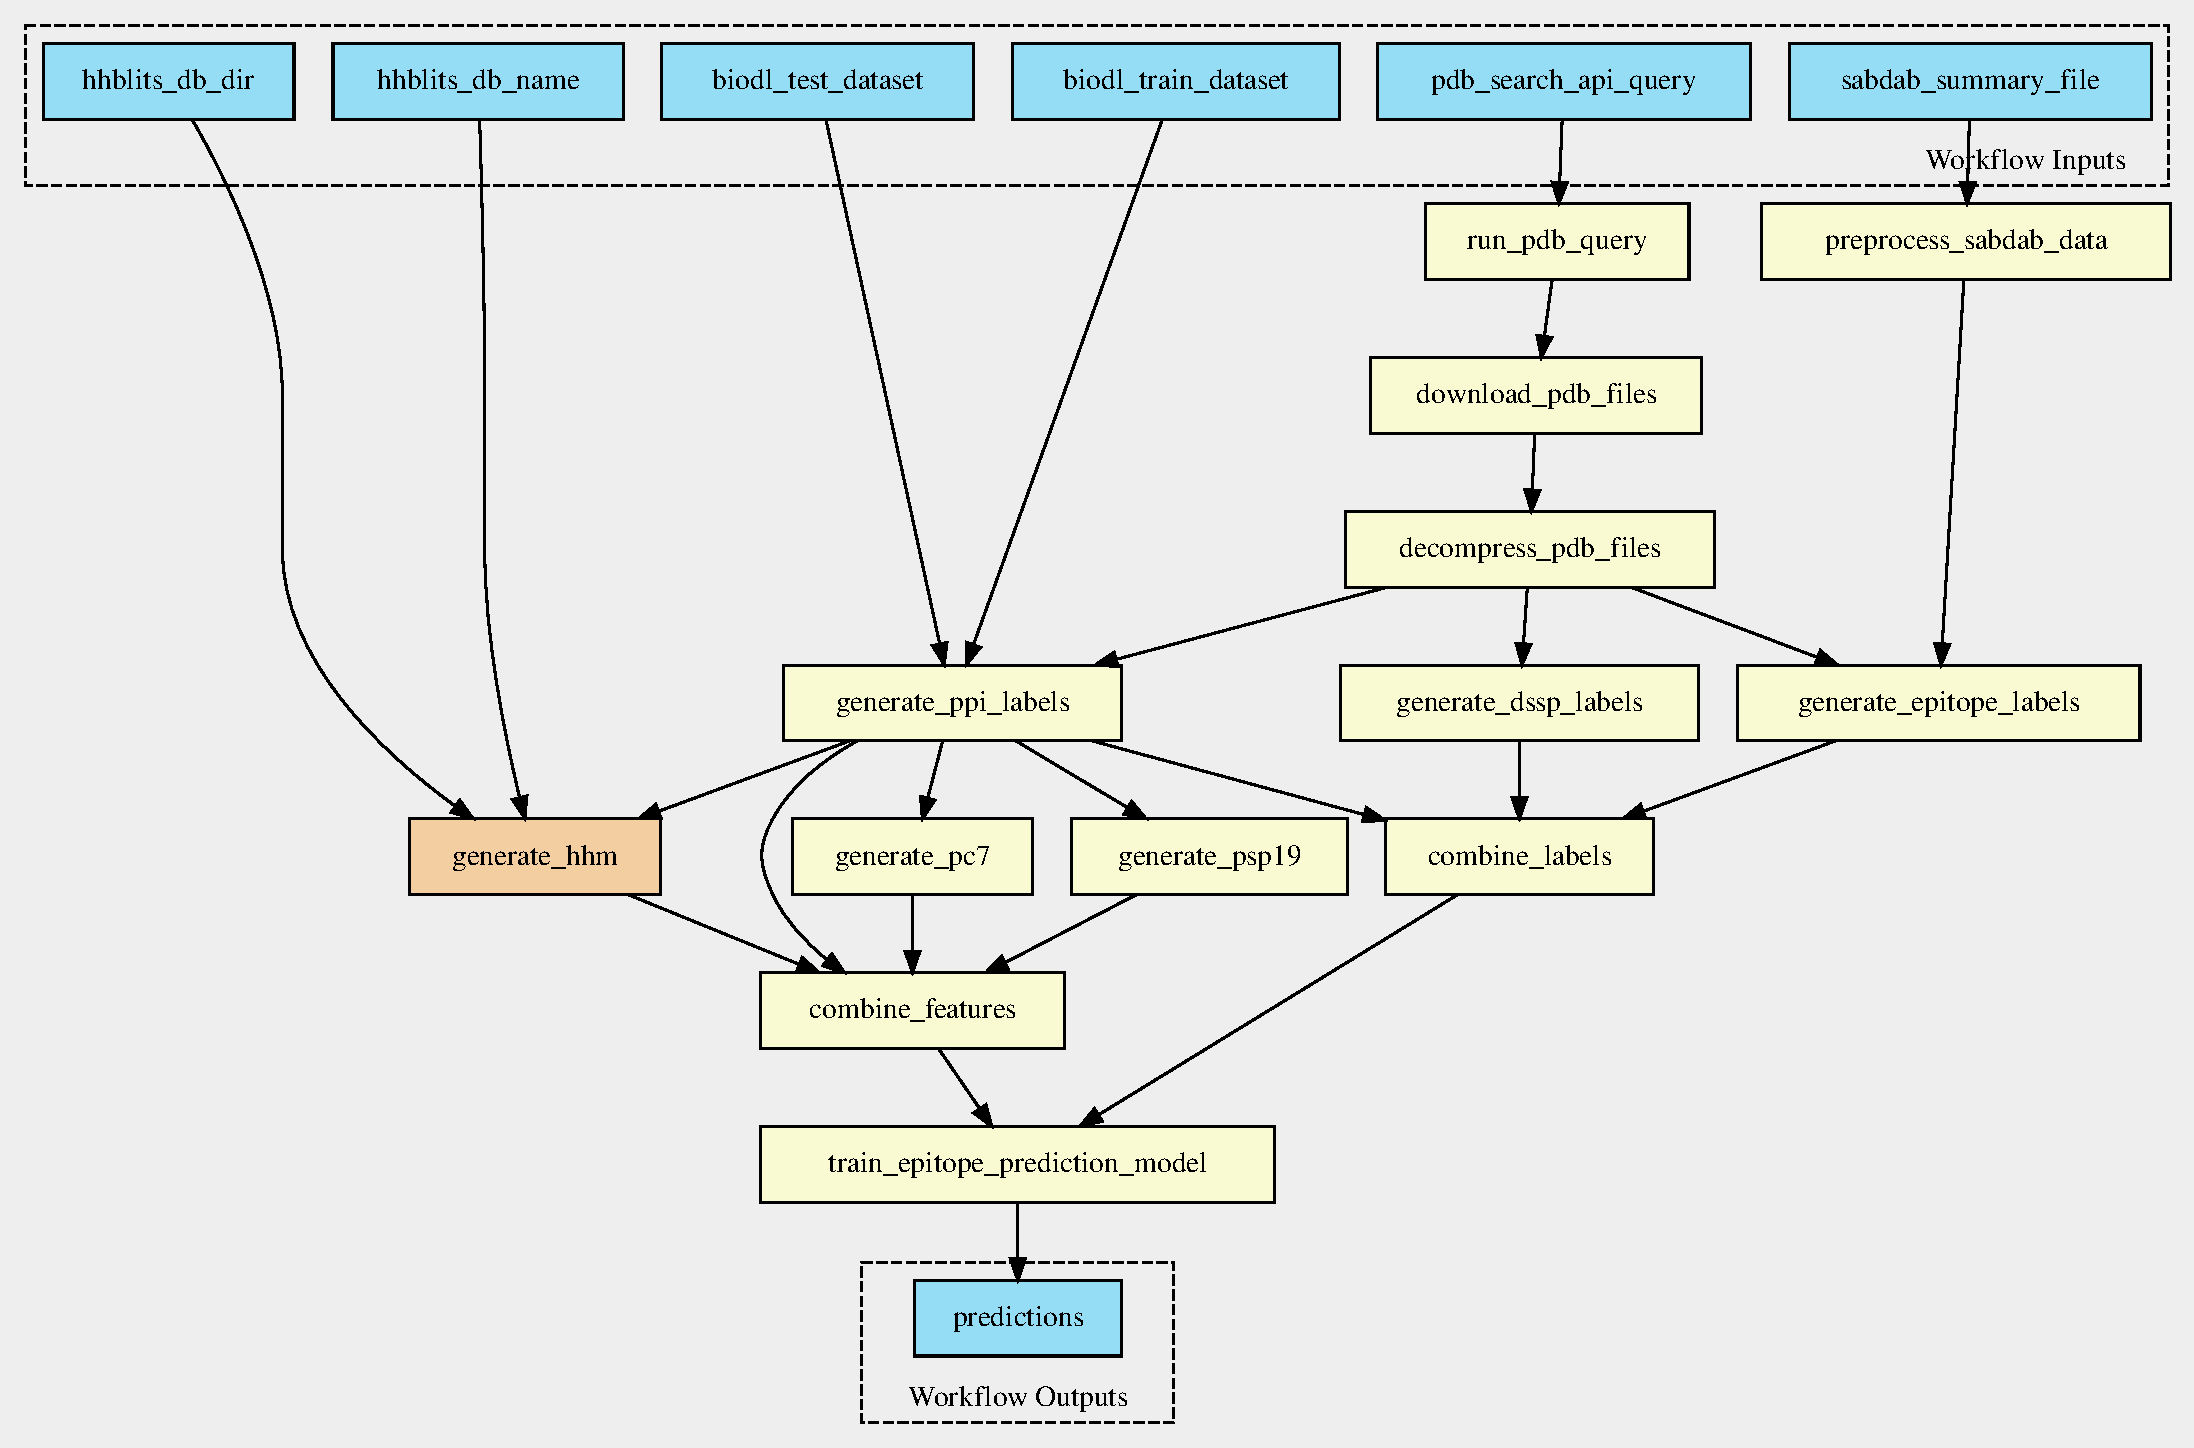
\includegraphics[width=1\linewidth]{taxonomy/workflow.pdf}
    \caption{CWL implementation of the workflow we used as an example. Based on data retrieved from multiple FAIR and non-FAIR resources, the workflow computes a set of input features and labels. These are subsequently used to train a deep learning model which predicts the amino acids in a protein which are likely to be \emph{epitopes}, i.e. binding sites for antibodies. Based on our experience, this workflow is exemplary for many problems which commonly arise when reproducing computational results.
    Nodes represent the steps, edges signify data flow between the steps. Yellow nodes indicate steps which run \emph{CommandLineTools}, orange nodes represent steps which control nested \emph{Workflows}, blue nodes signify workflow input and output parameters. }
    \label{fig:wf}
\end{figure*}
% \todorenske{We need to find a good term for this. \textit{Workflow template} was used in other publications (e.g. \citep{garijoDetectingCommonScientific2013}) for `workflow description' = the (CWL) document, which is not what we mean. \textit{Workflow motifs} are subcomponents of workflows, e.g. preprocessing \citep{garijoCommonMotifsScientific2014}. Workflow type? Workflow concept?} 


% \stodor{Explicitly reference figure 2 in the text}
As the basis of our provenance taxonomy, we used a type of bioinformatics workflow which was familiar to the authors: training a deep learning model to predict particular protein characteristics based on information encoded in the DNA. %\stodor{It is not really the DNA, but the protein sequence, but maybe this is less easy to understand.} 
More specifically, the model in our example predicts, for a given protein, which amino acids constitute \emph{epitopes}, i.e. binding sites for antibodies. Understanding antibody binding is important for e.g. vaccine design, but expensive and impractical to study experimentally because of the large number of possible protein-antibody combinations. However, the three-dimensional protein structure ultimately arises from the \emph{protein sequence}, which has been determined for a far greater number of proteins and in principle can be used to predict structural properties which are difficult to determine in the lab.
% Although this information could in principle be inferred by experimentally resolving the structure of the complex, in practice this is a difficult and expensive process and infeasible to perform for all complexes. Therefore, predictors have been developed to predict this information, based on patterns learned from protein sequence, which is encoded in the DNA and much easier to determine experimentally. 

% : training of a deep learning model on input features and labels derived from (experimental) data stored in large databases or previously published as standalone datasets. 

Based on our experience, the selected workflow has characteristics representative of many of the problems which commonly arise in reproducing computational processes. 1) It is a derived work; in our case the deep learning model is an adaptation of a previously published model for predicting general protein binding characteristics (the protein-protein interface) \cite{capelMultitaskLearningLeverage2022}. 2) Important data is the direct product of, or derived from, external databases which are continually updated and unlikely to return the same results when the same query is issued at a later date. Specifically, the property labels used to train the deep learning model are derived from experimentally resolved protein structures retrieved from large databases. 3) The workflow uses a variety of tools with specific versions, dependencies, and input parameter settings. 4) Finally, the development of this workflow involved many design choices, and many combinations of workflow steps and input configurations were tested during the search for an optimal configuration.

In our CWL description of the workflow (Figure \ref{fig:wf}), we aimed to optimize reproducibility by making some specific choices: We included database querying and data retrieval in the workflow and avoided the use of external identifier mapping tools, which are not likely to return the same output in the future. In addition, we executed most steps in software containers, and added structured annotations explaining the meaning of the workflow components and the data used as input. A detailed account of the workflow implementation can be found in the Supplementary Material (Section \emph{\nameref{sup:workflow}}). 

\subsection{Definition of Research Object use case scenarios}
\label{sec:stakeholders}

In this section, we describe the use cases of ROs associated with our example workflow coupled with the practitioners for which they are relevant. We consider five use cases, reflecting different stages in the workflow's lifetime. Some of these are applicable to workflows in most disciplines (e.g. U1), while at least one (U5) is specific to our exemplary workflow.
% \stodor{"Stages"? then use also in U3 \& U4, or nowhere. Also "stages" feel a bit linear.}

\begin{enumerate}[label=\textbf{U\arabic*}]
    \item \textbf{Workflow development}. Most relevant for: \textbf{Workflow author}. During this stage, the workflow design is not fully established. Different input datasets and configurations are tested. Steps may be added or removed based on the output of previous steps. ROs of multiple workflow runs may be used to compare different designs and configuration settings with each other. \label{uc:wf_dev}
    \item \textbf{Publishing the workflow}. Most relevant for: \textbf{Workflow author}. At this stage, the workflow is ready for publication, and the workflow author has to explain the methodology and rationale of the research in a scientific article, or write documentation for the workflow. The RO may serve as a guide during writing, comprising a record of used data and tools, contributions of collaborators (facilitating credit and attribution), and choices which were made during workflow development. \label{uc:writing}
    \item \textbf{Understanding the workflow}. Most relevant for: \textbf{Reader of the article describing the research}. This use case represents a stage in which an RO has been published in companionship with the article. The metadata contained in the RO serves as a bridge between the methods section of the article and the workflow itself. In addition, the metadata may connect the conclusions in the article to the results that support them. \label{uc:understanding}
    \item \textbf{Reproducing the workflow}. Most relevant for: \textbf{Third party continuing the research}. Follow-up stage after reading the article and examining the RO to understand the research (\ref{uc:understanding}). The RO is used as a guide to reproduce the analysis, before it is modified or extended for a new purpose. \label{uc:reproducing}
    \item \textbf{Model workflow execution as a service}. Most relevant for: \textbf{User of the trained model as a web service}. In this stage, the trained model has been made available as a web service, which can be used to predict epitopes for sequences for which the structure is unknown. An RO is the standard output format of the web-based tool. \label{uc:service}
\end{enumerate}


\subsection{Synthesis of a taxonomy of provenance}
% \todorenske{Same title as section, 1 of them should be changed.}

\label{sec:user_req}

Based on the use cases described in the previous section, we synthesized a list of \emph{provenance questions}, included in the Supplementary Material (Section \emph{\nameref{sup:provquestions}}).
Similar to the use case scenarios, we found that some questions are likely also relevant in most other domains, while others are highly specific for our workflow. Using our list of domain-informed provenance questions, we identified the metadata required to answer the questions and summarized this into a 6-component taxonomy of provenance types which should be represented in the provenance of the workflow execution: 


\begin{enumerate}[label=\textbf{T\arabic*}]
    \item \textbf{Scientific context}. Explanation of the choices which were made in the design of the workflow and parameter values. \label{tax:context}
    \item \textbf{Data}. Input and (intermediate) output data.\label{tax:data} % To explain meaning and context of the data as well as describe data not included in RO for storage, security, or privacy reasons. 
    \item \textbf{Software}. The tools directly orchestrated by the workflow, and their dependencies. \label{tax:software} % Facilitates reproduction of workflow at a later time or helps finding an alternative tool in the case of code rot. 
    \item \textbf{Workflow}. The (CWL) workflow and tool descriptions. \label{tax:wf} % Workflows are software and can be reused when published in a workflow repository.
    \item \textbf{Computational environment}. Metadata about the system on which the workflow was executed, comprising both software and hardware. \label{tax:env} % Necessary for reproduction of the workflow execution.
    \item \textbf{Execution details}. Additional information about the workflow execution itself. \label{tax:execution}
\end{enumerate}
\begin{table*}
\caption{Overview of provenance taxonomy, with the provenance questions (\emph{PQs}) that apply to each of the categories. In addition, the components of the taxonomy are integrated with already accepted principles and guidelines (\emph{Source}).
%\todorenske{What should go in Refs? Only officially defined standards like FAIR principles/data citation principles or also random publications which mention that including something may be necessary?}
}\label{tab:taxonomy}
% Use "S" column identifier (from siunitx) to align on decimal point.
% Use "L", "R" or "C" column identifier for auto-wrapping columns with tabularx.

\begin{tabularx}{\linewidth}{p{0.1in}p{0.3in}p{1.3in}Lp{0.45in}p{0.3in}} %{l{0.05\textwidth} l{0.3\textwidth} l{0.5\textwidth} L{0.05\textwidth} l{0.05\textwidth} l{0.05\textwidth}}
\toprule
{Type} & {Subtype} & {Name} & {Metadata}  & {PQs} & {Source} \\
\midrule
T1  & {SC1}\label{tax:sc1}   & Workflow design  & Annotations on the design of the workflow and its components. Purpose of the workflow, why steps were included or excluded, the meaning of particular input parameters, etc.    & 1-2, 11-12, 25-27    & \citep{committeeonreproducibilityandreplicabilityinscienceReproducibilityReplicabilityScience2019,belhajjameResearchObjectSuite2014,grykWorkflowsProvenanceInformation2017,stoddenEnhancingReproducibilityComputational2016}   \\
    & SC2   & Entity annotations                & The meaning of individual input and output data entities. Why were they chosen? How are the results interpreted?          & 1-5, 13, 28-29, 67-69  &   \\
    & SC3   & Workflow execution annotations    & Annotations about a set of parameters in a particular workflow run. Allows to distinguish between the ROs of multiple workflow runs.             & 6-7, 30-31 &  \\
\midrule
T2  & D1    & Data identification               & Persistent identifier (PID), version, name and description of the dataset. Preferred citation of the data. \emph{When the data is not FAIR:} URL and download date as an alternative for PID and version. \emph{When the dataset is a subset of a larger collection (e.g. a database):} PID of database, database version and download date, and the query or filtering strategy which produced the dataset.    & 13-16, 32-36, 47, 67-69 & \citep{datacitationsynthesisgroupJointDeclarationData2014} \\
    & D2    & File characteristics              & Filename, format, creation and last modification timestamps, size, and checksum.  & 15, 48  &  \\
    & D3    & Data access                       & URL to a downloadable form of the data. License.   &  8, 49  & \\
    & D4    & Parameter mapping                 & The workflow and step parameters for which the data is an input or output.   & 37-38 &   \\
\midrule
T3  & SW1   & Software identification           & PID, name, version, release date and description of the software. Preferred citation. \textit{When the software is not FAIR:} URL of repository, download date and/or git commit hash as substitute for PID, version or release date.       &  16-20, 50     &   \citep{smithSoftwareCitationPrinciples2016} \\
    & SW2   & Software documentation            & URL of documentation or other metadata which is important to make informed use of the tool. URL to repository with source code of the software. &  39-40, 51-52  & \\
    & SW3   & Software access                   & URL to downloadable, executable form of the software. License.               &  9, 53  & \\
\midrule
T4  & WF1   & General software metadata         & At workflow and step level, according to T3.                 & 12, 21-23, 41, 70 & \citep{gobleFAIRComputationalWorkflows2020}\\
    & WF2   & Workflow parameters               & Type, format, and description, at workflow and step-level.                & 42-44  & \\
    & WF3   & Workflow requirements             & Software and hardware resources which are required to execute the workflow or workflow steps. &  54-56  & \\
\midrule
T5  & ENV1  & Software environment              & Software (dependencies), operating system. Dependencies could comprise all installed software (might contain much redundant information if a step was not executed in a software container), or the dependencies of the software which is run (which may be difficult to identify). Should follow the requirements as described in T3.       &    57     &  \citep{committeeonreproducibilityandreplicabilityinscienceReproducibilityReplicabilityScience2019}  \\
    & ENV2  & Hardware environment              & Available RAM, storage, number and type of CPUs and GPUs. Network access.       &    58        & \\
    & ENV3  & Container image                   & Image name, tag and digest (because names and tags are not stable). Additional metadata (extracted from image labels), contents of Dockerfile (if built from Dockerfile), and general requirements for software as described in SW1.                & 24, 59-60 &  \\
\midrule
T6  & EX1   & Execution timestamps              & When the workflow was executed, at step-granularity. The timestamps can be helpful when files were downloaded during the execution, especially from a database which does not have clear versions. In addition, the duration of the execution may be important during workflow development (test different settings) and when reproducing the workflow. & 1-5, 10, 61-63 &   \\
    & EX2   & Consumed resources             & The resources used during execution, at step-granularity. This is different from what was described in WF3, because there we only described what was available, not what was actually used.  & 7, 64  &  \\
    & EX3   & Workflow engine                   & Software, therefore with same metadata as general software entities (T3).             & 45, 65 & \\
    & EX4   & Human agent                       & At a minimum, a PID such as ORCID should be included, or name and email of the person who ran the workflow. These details may be important for attribution (U2), and can also be used by third parties to ask further questions about the research.                 & 46, 66 &  \\
\bottomrule
\end{tabularx}


% \begin{tablenotes}
% \item Source is from this website: \url{https://www.sedl.org/afterschool/toolkits/science/pdf/ast_sci_data_tables_sample.pdf}
% \end{tablenotes}
\end{table*}

Each component of the taxonomy consists of several subcomponents, which are outlined in Table \ref{tab:taxonomy}.